\documentclass[xcolor={usenames,dvipsnames}]{beamer}

\mode<presentation> { }

\usetheme{metropolis}
\usepackage{listings}
\usepackage{polyglossia}
\setmainlanguage{english}


\usepackage[numbers]{natbib}

\usepackage{tikz}
\usetikzlibrary{arrows, decorations.pathmorphing,backgrounds,fit,positioning,shapes.symbols,chains, positioning,automata}

\usepackage{lstc}
\usepackage{lstnasm}
\renewcommand{\lstcurrentinputdir}{listings}

%settings 
\everymath{\displaystyle}

\title{Dynamic libraries explained }
\subtitle{as seen by a low-level programmer}
\author{I.Zhirkov}

\date{2017}

\AtBeginSection[]{
    \begin{frame}<beamer>{}
        {\huge \secname}
    \end{frame}
}
%\AtBeginSection[]
%{
%  \begin{frame}<beamer>{\secname}
%    \tableofcontents[currentsubsection,
%      subsectionstyle=show/show/hide, sectionstyle=hide/hide]
%  \end{frame}
%}
%

\begin{document}

\begin{frame}
  \titlepage
\end{frame}


\begin{frame}{Exemplary environment}
    \begin{itemize} 
        \item  Intel 64 aka AMD64 aka x86\_64.
        \item  GNU/Linux
        \item  Object file format: ELF files.
\end{itemize} 
\end{frame}


\section{Preface}
\begin{frame}{Compilation pipeline}
    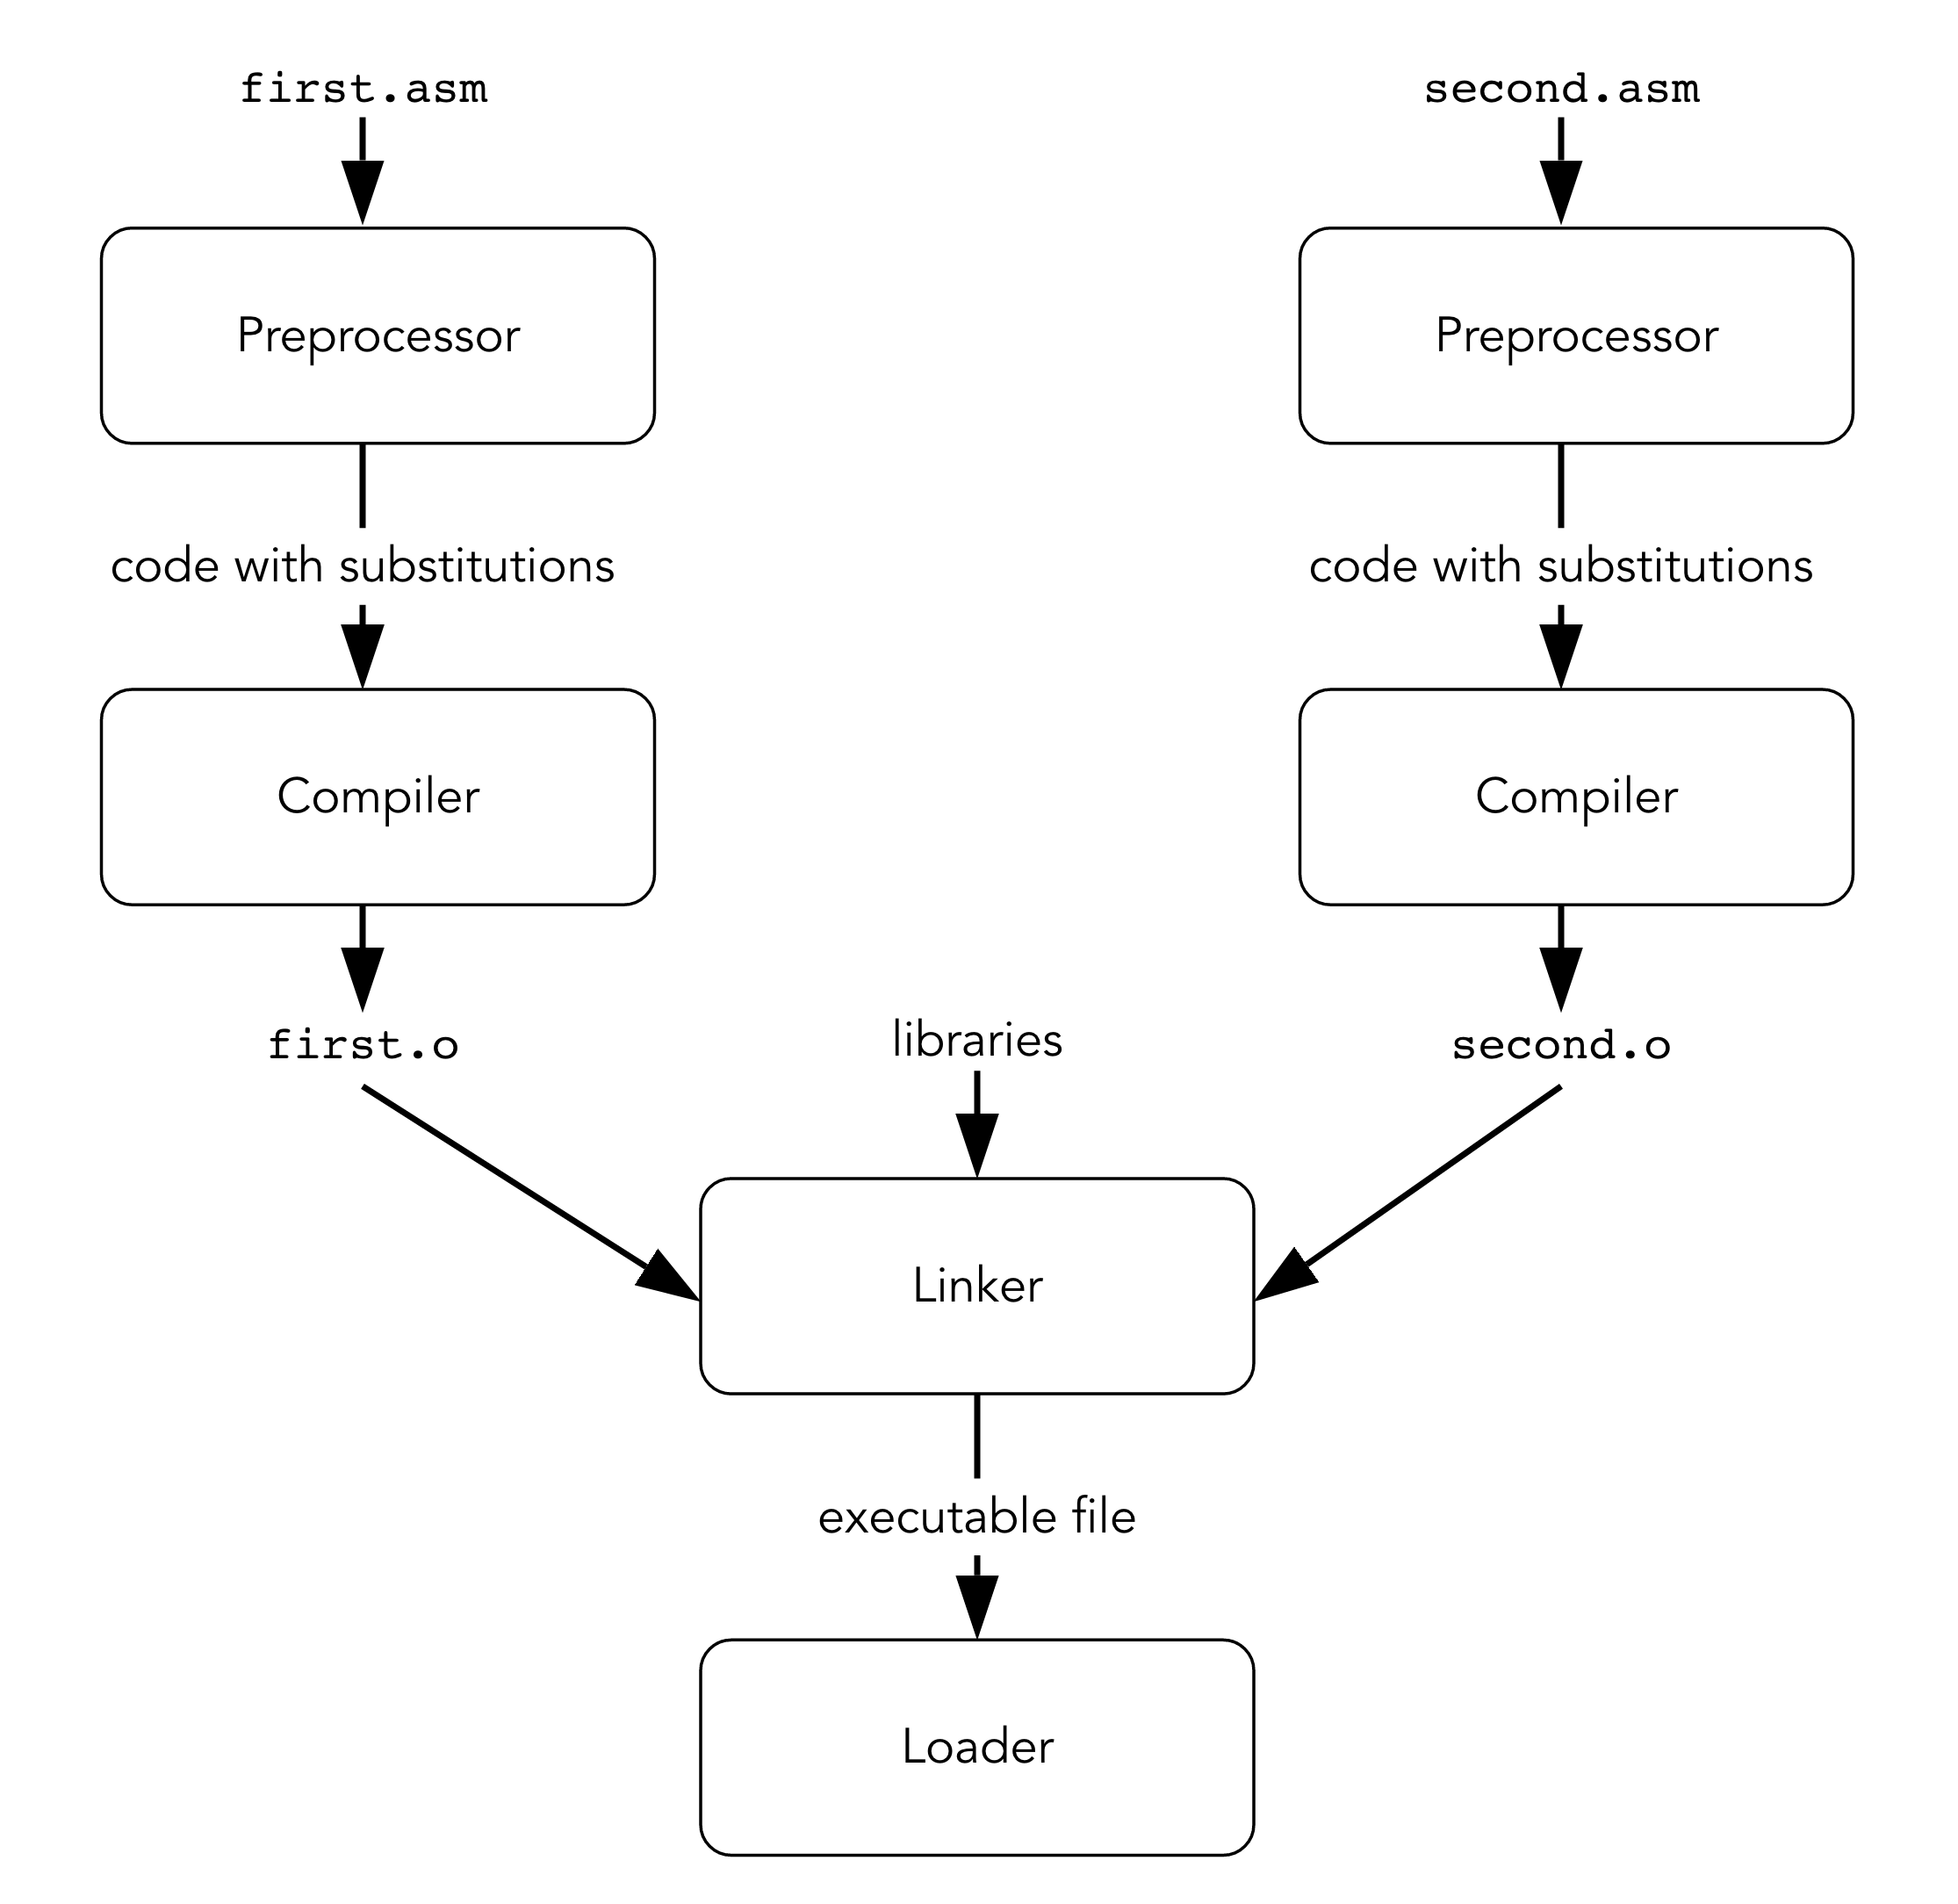
\includegraphics[height=\textheight]{images/compilation.png} 
\end{frame}


\begin{frame}{Particular interest}

\begin{itemize}
    \item  Separate compilation.
    \item  Using a separate program (linker) on the final stage.
\end{itemize}
\end{frame}

\begin{frame}{Why we need separate compilation?}
\begin{itemize}
    \item  Use code that is already compiled.
    \item  Don't recompile everything after each change.

    \begin{itemize}
        \item  Some programs take \emph{hours} to compile.
    \end{itemize}
    
\end{itemize}

\end{frame}
%\begin{frame}[allowframebreaks]
%\frametitle{References}
%\bibliography{biblio} 
%\end{frame}

\end{document}


